\documentclass[12pt,a4paper]{article}

\usepackage[T1]{fontenc}
\usepackage[utf8]{inputenc}
\usepackage[english]{babel}
\usepackage{amsmath,amssymb}
\usepackage{geometry}
\usepackage{graphicx}
\usepackage{hyperref}
\usepackage{booktabs}
\usepackage{tikz}
\usetikzlibrary{patterns, arrows.meta, decorations.markings}

\geometry{margin=2.5cm}

\title{Dynamics and Optimization of Rifle Barrel Vibrations \\ \large From ballistic theory to finite-element simulation}
\author{}
\date{}

\begin{document}

	\maketitle
	\tableofcontents
	\vspace{1cm}

	\section{Introduction: principles of positive compensation}
	\label{sec:intro}

	This first section presents the \emph{why} and the \emph{how} of positive compensation without resorting to mathematical tools. A curious reader who only wishes to understand the idea and its practical interest may stop at the end of section~\ref{sec:plan}; the subsequent sections then develop the rigorous modelling and the numerical simulation.

	\subsection{The challenge of precision shooting}

	In precision-shooting disciplines (for instance, ISSF 50-metre prone), the pursuit of a perfect group runs up against the physical limits of the ammunition. Even with \emph{match}-grade cartridges, there remains an unavoidable variation in muzzle exit velocity --- the \emph{muzzle velocity} --- from one cartridge to the next. This variation, often measured in feet per second (fps), is typically on the order of a few percent.

	\subsection{Why a variation in velocity moves the point of impact}

	A slower bullet spends more time in flight to reach the target and therefore suffers gravitational acceleration for longer: it drops more. Mechanically, on target, this translates into a lower impact than a faster bullet fired with the same setting. If the barrel were a perfectly rigid and stationary tube, the velocity spread of the cartridges would inevitably translate into a \emph{vertical streak} on the target: fast bullets at the top, slow ones at the bottom.

	\subsection{The barrel vibrates like a tuning fork}

	In reality, when the shot is fired, the barrel does not stay still: it begins to vibrate. The powder explosion, the recoil of the firearm, the projectile's travel through the bore and its friction against the rifling all excite transverse oscillations --- that is, up-and-down and side-to-side --- that move the muzzle by a few hundredths of a degree, in the manner of a tuning fork ringing after being struck. These vibrations last several tens of milliseconds, well beyond the time it takes for the bullet to travel through the barrel (typically 2 to 3 milliseconds).

	During those 2 to 3 milliseconds, the muzzle is therefore in motion: it rises, falls, returns through its equilibrium position, and so on. The exact angle at which the bullet exits depends not only on the shooter's aim, but also on the \emph{precise instant} of exit.

	\subsection{What sets the magnitude of the vibrations}

	Where does this motion come from? The dominant source, emphasised by G.\ Kolbe~\cite{KolbeSim}, is \emph{recoil}: under the thrust of the gases, the whole firearm moves backwards and \emph{rotates about its centre of gravity}. The barrel axis (the bore line, through which the bullet exits) lies \emph{above} that centre of gravity; the recoil thrust therefore acts with a \emph{lever arm} and imparts a couple to the rear of the barrel, exactly as a flick delivered off-centre tips a ruler lying on a table. This couple is the ``hammer blow'' that makes the tuning fork ring.

	Two concrete quantities then govern the \emph{amplitude} of the muzzle motion:
	\begin{itemize}
		\item the \textbf{total weight of the firearm}: a heavy rifle absorbs recoil while moving less, and therefore vibrates less;
		\item the \textbf{height of the bore above the centre of gravity}: the larger this lever arm, the larger the couple --- and hence the amplitude.
	\end{itemize}
	Neither parameter appears in the tuner setting (which acts on the \emph{rhythm} of the vibrations, not on their cause), but together they explain why two rifles with identical barrels but different mountings do not tune the same way. They are reintroduced formally in Section~\ref{sec:excitation} as the excitation moment $M_0(t)$.

	\subsection{The principle of positive compensation}

	The brilliant idea, proposed as early as 1901 by A.\ Mallock~\cite{Mallock} and formalised for modern shooting by G.\ Kolbe (Border Barrels)~\cite{Kolbe,KolbeWeb}, is to \emph{exploit} these vibrations rather than suffer them. If one manages to tune the barrel so that the muzzle is \emph{rising} at the precise moment the bullet leaves it, then:

	\begin{itemize}
		\item a \textbf{fast} bullet exits slightly \emph{early}: at that moment, the barrel has not yet had time to rise much, and the bullet is launched at a \emph{lower} angle (figure~\ref{fig:compensation_positive}, red trajectory);
		\item a \textbf{slow} bullet exits slightly \emph{late}: the barrel has continued to rise, and the bullet is launched at a \emph{higher} angle (blue trajectory).
	\end{itemize}

	The slow bullet is therefore projected \emph{higher} initially; on target, its extra drop (because it spent longer in flight) is exactly compensated by its extra starting height. All bullets, fast or slow, can thus end up at the \emph{same} point of impact. This is what Kolbe calls \emph{positive compensation}.

	\begin{figure}[!htb]
		\centering
		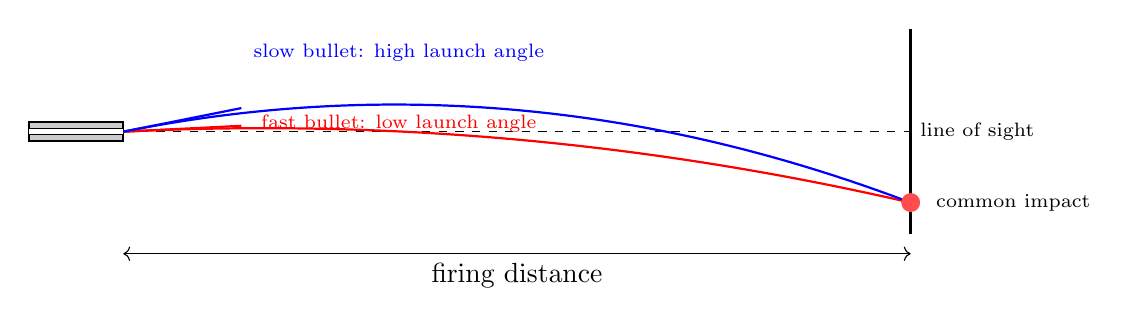
\begin{tikzpicture}[x=1cm, y=1cm]
			% Barrel (mini)
			\draw[thick, fill=gray!40] (-1.2, -0.12) rectangle (0, 0.12);
			\draw[fill=white] (-1.2, -0.04) rectangle (0, 0.04);
			% Line of sight
			\draw[dashed, thin] (0, 0) -- (10, 0);
			\node[anchor=west] at (10, 0) {\scriptsize line of sight};
			% Fast bullet trajectory (low angle)
			\draw[red, thick, domain=0:10, samples=80]
				plot (\x, {0.05*\x - 0.014*\x*\x});
			% Slow bullet trajectory (higher angle)
			\draw[blue, thick, domain=0:10, samples=80]
				plot (\x, {0.20*\x - 0.029*\x*\x});
			% Target
			\draw[very thick] (10, -1.3) -- (10, 1.3);
			\fill[red!70] (10, -0.9) circle (0.12);
			\node[anchor=west] at (10.2, -0.9) {\scriptsize common impact};
			% Muzzle angles illustrated
			\draw[red, thick] (0, 0) -- (1.5, 0.075);
			\draw[blue, thick] (0, 0) -- (1.5, 0.30);
			\node[red] at (3.5, 0.1) {\scriptsize fast bullet: low launch angle};
			\node[blue] at (3.5, 1.0) {\scriptsize slow bullet: high launch angle};
			% Distance D
			\draw[<->] (0, -1.55) -- (10, -1.55);
			\node[below] at (5, -1.55) {firing distance};
		\end{tikzpicture}
		\caption{Geometric principle of positive compensation. If the muzzle is rising when the bullets exit, the slower bullets (which leave later) benefit from a higher launch angle. Their extra starting height compensates the extra drop due to their longer flight, and all bullets can end up at the same point of impact on target.}
		\label{fig:compensation_positive}
	\end{figure}

	\subsection{The role of the tuner}

	For this phenomenon to occur, one still needs to \emph{match} the barrel's vibrations to the bullet's exit time --- hence the term \emph{tuner}, which denotes a movable mass (typically 100 to 400 grams) fixed to the muzzle of the barrel. By screwing this mass in or out, the shooter moves it closer to or farther from the muzzle, which subtly modifies the barrel's vibration frequency. This amounts to adjusting the rhythm of the ``tuning fork'': one lengthens or shortens the time it takes for the muzzle to return through its equilibrium position, so that this instant falls precisely when the average bullet exits.

	Any change of ammunition or even of lot in principle requires a new adjustment, since the average velocity --- and therefore the barrel travel time --- changes. Shooters typically proceed by successive trials (the so-called \emph{ladder} or \emph{Audette} method~\cite{Audette}): one fires several series while changing the tuner position by one notch each time, and retains the position for which the groups are tightest.

	\subsection{Intuitive summary}

	In summary, positive compensation requires three ingredients:
	\begin{enumerate}
		\item a barrel that vibrates enough to move noticeably between the exit of a fast bullet and that of a slow bullet;
		\item a \emph{tuning} of these vibrations that places the exit time of the average bullet at the right point of the oscillation (the \emph{rising} phase);
		\item a quantitative compromise between the angular speed of the motion and the ballistic drop: a barrel that rises too slowly will not compensate enough for the dispersion, and a barrel that rises too fast will over-compensate.
	\end{enumerate}
	The following sections formalise each of these three ingredients and show how the physical parameters of the barrel, the tuner and the ammunition combine to reach the optimum.

	\subsection{Document outline}
	\label{sec:plan}

	The remainder of the document develops the theory and the simulation:
	\begin{itemize}
		\item Section~\ref{sec:notations}: list of notations and conventions used.
		\item Section~\ref{sec:math}: mathematical modelling of the barrel (Euler-Bernoulli beam, finite-element method, Newmark-$\beta$ time integration).
		\item Section~\ref{sec:modale}: analysis of natural frequencies and sensitivity to the tuner.
		\item Section~\ref{sec:cinematique}: mathematical criterion of positive compensation, distinction between temporal node and antinode, experimental confirmation by Kolbe, and validation by the numerical simulation.
		\item Section~\ref{sec:conclusions}: practical conclusions for the shooter.
	\end{itemize}

	\section{Notations and conventions}
	\label{sec:notations}

	We adopt the SI system of units ($\text{m}, \text{kg}, \text{s}, \text{Pa}, \text{rad}$). The $x$-axis is aligned with the bore of the barrel, oriented from the breech ($x=0$) toward the muzzle ($x=L$). The $y$-axis is transverse, oriented upward. Unless otherwise stated, angles are in radians; the usual conversions are
	\(1\ \text{MOA} = \pi/(180 \times 60)\ \text{rad} \approx 2.909 \times 10^{-4}\ \text{rad}\) and
	\(1\ \text{mrad} \approx 3.438\ \text{MOA}.\)

	\begin{center}
		\renewcommand{\arraystretch}{1.12}
		\begin{tabular}{l l l}
			\toprule
			Symbol & Meaning & Unit \\
			\midrule
			\multicolumn{3}{l}{\emph{Barrel geometry and material}} \\
			$L$ & Barrel length & m \\
			$D_\text{ext}, D_\text{int}$ & Outer (profile) and inner (bore) diameters & m \\
			$A$ & Cross-sectional area $\tfrac{\pi}{4}(D_\text{ext}^2 - D_\text{int}^2)$ & m$^2$ \\
			$I$ & Second moment of area $\tfrac{\pi}{64}(D_\text{ext}^4 - D_\text{int}^4)$ & m$^4$ \\
			$E$ & Young's modulus (steel $\approx 200$ GPa) & Pa \\
			$\rho$ & Mass density (steel $\approx 7850$ kg/m$^3$) & kg/m$^3$ \\
			$EI$ & Flexural rigidity & N$\cdot$m$^2$ \\
			$\rho A$ & Mass per unit length & kg/m \\
			\midrule
			\multicolumn{3}{l}{\emph{Beam kinematics}} \\
			$y(x,t)$ & Transverse deflection at point $x$ and time $t$ & m \\
			$\theta(x,t) \equiv \partial y/\partial x$ & Slope / angle of the neutral axis & rad \\
			$\theta(L,t)$ & Angle at the muzzle (launch angle) & rad \\
			$\dot\theta = \partial \theta/\partial t$ & Muzzle angular velocity & rad/s \\
			\midrule
			\multicolumn{3}{l}{\emph{Tuner}} \\
			$m_t$ & Tuner mass (typically 100--400 g) & kg \\
			$J_t$ & Tuner transverse moment of inertia & kg$\cdot$m$^2$ \\
			\midrule
			\multicolumn{3}{l}{\emph{Natural modes}} \\
			$\omega_n$ & Angular natural frequency of mode $n$ & rad/s \\
			$f_n = \omega_n/(2\pi)$ & Natural frequency of mode $n$ & Hz \\
			$T_n = 1/f_n$ & Natural period of mode $n$ & s \\
			$\phi_n(x)$ & Spatial shape of mode $n$ & --- \\
			$\zeta_n$ & Modal damping ratio & --- \\
			\midrule
			\multicolumn{3}{l}{\emph{Projectile and internal ballistics}} \\
			$m_p$ & Projectile mass (.22 LR: $\approx 2.6$ g) & kg \\
			$v(x,t)$ & Projectile velocity at position $x$ & m/s \\
			$v_0, v_\text{muzzle}$ & Muzzle velocity (at exit) & m/s \\
			$\bar v$ & Effective average velocity in the barrel & m/s \\
			$t_b$ & Projectile travel time in the barrel & s \\
			$p(t)$ & Pressure in the chamber / bore & Pa \\
			$A_\text{bore} = \tfrac{\pi}{4} D_\text{int}^2$ & Effective cross-sectional area of the bore & m$^2$ \\
			$\tau_v \equiv -\partial t_b/\partial v_0$ & Sensitivity of exit time to muzzle velocity & s/(m/s) \\
			\midrule
			\multicolumn{3}{l}{\emph{Target and compensation}} \\
			$D$ & Shooting distance (50 m for ISSF prone) & m \\
			$g$ & Gravitational acceleration ($\approx 9.81$ m/s$^2$) & m/s$^2$ \\
			$h_\text{bal}(v_0)$ & Ballistic drop at distance $D$ & m \\
			$\theta_\text{out}$ & Muzzle angle at instant $t_b$: $\theta(L, t_b)$ & rad \\
			$\dot\theta_\text{out}^\star$ & \emph{Target} angular velocity for full compensation & rad/s \\
			\midrule
			\multicolumn{3}{l}{\emph{Numerical simulation}} \\
			$N$ & Number of finite elements & --- \\
			$L_e = L/N$ & Element length & m \\
			$[K], [M], [C]$ & Global stiffness, mass, damping matrices & --- \\
			$\{u(t)\}$ & Vector of nodal DOFs (translations + rotations) & --- \\
			$\Delta t$ & Newmark-$\beta$ time step & s \\
			$\gamma, \beta$ & Newmark scheme parameters & --- \\
			$h_\text{offset}$ & Recoil-moment lever arm at the breech (excitation) & m \\
			\bottomrule
		\end{tabular}
	\end{center}

	\section{Mathematical development}
	\label{sec:math}

	\subsection{Continuous model: Euler--Bernoulli beam}

	We model the barrel as a prismatic beam clamped at the breech ($x=0$) and free at the muzzle ($x=L$), with cross-sectional area $A(x)$ and second moment of area $I(x)$ (assumed piecewise constant; \emph{bull}, \emph{sporter} and tapered profiles can be handled by varying these element-wise). Writing $y(x,t)$ for the transverse deflection, the partial differential equation governing small oscillations reads:
	\begin{equation}
		\label{eq:EB}
		\rho A \,\frac{\partial^2 y}{\partial t^2} \;+\; \frac{\partial^2}{\partial x^2}\!\left(EI \,\frac{\partial^2 y}{\partial x^2}\right) \;=\; q(x,t),
	\end{equation}
	where $q(x,t)$ represents the distributed transverse load. The boundary conditions are:
	\begin{equation*}
		y(0,t) = 0,\qquad \frac{\partial y}{\partial x}(0,t) = 0,\qquad EI\,\frac{\partial^2 y}{\partial x^2}\bigg|_{x=L}\!\! = M_t,\qquad \frac{\partial}{\partial x}\!\left(EI\,\frac{\partial^2 y}{\partial x^2}\right)\bigg|_{x=L}\!\! = -F_t,
	\end{equation*}
	where $M_t$ and $F_t$ respectively denote the moment and the force applied by the tuner (including its inertial effects). For a thick-walled match profile, the Euler--Bernoulli assumption (plane sections remaining plane and normal to the neutral axis) is reasonable as long as $L/D_\text{ext} \gtrsim 20$; beyond that, a Timoshenko model accounting for rotational inertia and shear deformation is preferable.

	\begin{figure}[!htb]
		\centering
		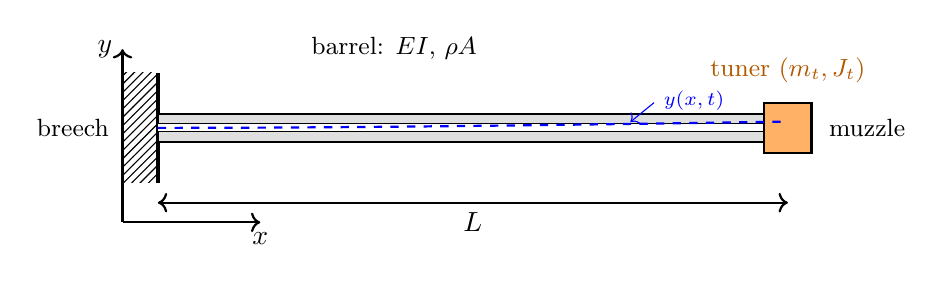
\begin{tikzpicture}[x=1cm, y=1cm]
			% Clamping wall (hatched)
			\fill[pattern=north east lines] (-0.45, -0.7) rectangle (0, 0.7);
			\draw[very thick] (0, -0.7) -- (0, 0.7);
			% Barrel
			\draw[thick, fill=gray!25] (0, -0.18) rectangle (8, 0.18);
			\draw[fill=white] (0, -0.05) rectangle (8, 0.05);
			% Tuner (ring at muzzle)
			\draw[thick, fill=orange!60] (7.7, -0.32) rectangle (8.3, 0.32);
			% Length L
			\draw[<->, thick] (0, -0.95) -- (8, -0.95);
			\node[below] at (4, -0.95) {$L$};
			% Labels
			\node[anchor=south] at (3, 0.75) {\small barrel: $EI$, $\rho A$};
			\node[anchor=south, orange!70!black] at (8, 0.45) {\small tuner $(m_t, J_t)$};
			\node[anchor=east] at (-0.5, 0) {\small breech};
			\node[anchor=west] at (8.4, 0) {\small muzzle};
			% Axes
			\draw[->, thick] (-0.45, -1.2) -- (-0.45, 1.0) node[left] {$y$};
			\draw[->, thick] (-0.45, -1.2) -- (1.3, -1.2) node[below] {$x$};
			% Illustrative deformed shape (dashed)
			\draw[blue, thick, dashed, domain=0:8, samples=50]
				plot(\x, {0.12*(\x/8)^2 - 0.04*(\x/8)^3});
			% Deflection label with arrow to curve
			\node[blue, anchor=west] at (6.3, 0.35) {\scriptsize $y(x,t)$};
			\draw[blue, thin, ->] (6.3, 0.32) -- (6.0, 0.075);
		\end{tikzpicture}
		\caption{Barrel model: Euler-Bernoulli beam clamped at the breech ($x=0$), free at the muzzle ($x=L$), carrying at its end a point mass and its rotational inertia $(m_t, J_t)$ representing the tuner. The dashed curve illustrates a transverse deflection $y(x,t)$.}
		\label{fig:schema_canon}
	\end{figure}

	\subsection{Finite-element discretisation}

	We seek a weak solution of \eqref{eq:EB}. Multiplying by a test function $w(x)$ of class $\mathcal{C}^1$ satisfying the essential conditions and integrating by parts twice over $[0,L]$, one obtains the \emph{variational formulation}:
	\begin{equation}
		\label{eq:weak}
		\int_0^L \rho A \,\ddot y\, w \,\mathrm{d}x \;+\; \int_0^L EI\, y'' w'' \,\mathrm{d}x \;=\; \int_0^L q\,w\,\mathrm{d}x \;+\; [\text{boundary terms}].
	\end{equation}

	The barrel is partitioned into $N$ elements of length $L_e$. On each element, two degrees of freedom are assigned per node: deflection $y$ and rotation $\theta = y'$. The local field $y_e(\xi)$, where $\xi \in [0,L_e]$ is the local coordinate, is expressed using \textbf{cubic Hermite shape functions}:
	\begin{equation}
		\label{eq:hermite}
		y_e(\xi) = \mathbf{N}(\xi)\, \mathbf{u}_e, \qquad \mathbf{u}_e = \begin{pmatrix} y_1 \\ \theta_1 \\ y_2 \\ \theta_2 \end{pmatrix},
	\end{equation}
	with
	\begin{align*}
		N_1(\xi) &= 1 - 3\bar\xi^2 + 2\bar\xi^3, & N_2(\xi) &= L_e\,(\bar\xi - 2\bar\xi^2 + \bar\xi^3), \\
		N_3(\xi) &= 3\bar\xi^2 - 2\bar\xi^3, & N_4(\xi) &= L_e\,(-\bar\xi^2 + \bar\xi^3),
	\end{align*}
	where $\bar\xi = \xi/L_e$. These polynomials guarantee the $\mathcal{C}^1$ continuity at the nodes required by the biharmonic operator of \eqref{eq:weak}.

	Substituting \eqref{eq:hermite} into \eqref{eq:weak}, one obtains, for each element, the elementary stiffness matrix
	\begin{equation}
		[K]^e \;=\; \int_0^{L_e} EI\, (\mathbf{N}'')^{\!\top} \mathbf{N}'' \,\mathrm{d}\xi
		\;=\; \frac{EI}{L_e^3}
		\begin{bmatrix}
			12     & 6L_e   & -12    & 6L_e   \\
			6L_e   & 4L_e^2 & -6L_e  & 2L_e^2 \\
			-12    & -6L_e  & 12     & -6L_e  \\
			6L_e   & 2L_e^2 & -6L_e  & 4L_e^2
		\end{bmatrix},
	\end{equation}
	and the consistent mass matrix
	\begin{equation}
		[M]^e \;=\; \int_0^{L_e} \rho A\, \mathbf{N}^{\!\top} \mathbf{N} \,\mathrm{d}\xi
		\;=\; \frac{\rho A L_e}{420}
		\begin{bmatrix}
			156    & 22L_e  & 54     & -13L_e \\
			22L_e  & 4L_e^2 & 13L_e  & -3L_e^2 \\
			54     & 13L_e  & 156    & -22L_e \\
			-13L_e & -3L_e^2 & -22L_e & 4L_e^2
		\end{bmatrix}.
	\end{equation}
	The nodal load vector is obtained analogously as $\mathbf{f}_e = \int_0^{L_e} q(\xi,t)\, \mathbf{N}^{\!\top}\,\mathrm{d}\xi$.

	\subsection{Assembly, boundary conditions and tuner integration}

	The global matrices $[K]$ and $[M]$ of size $2(N+1) \times 2(N+1)$ are assembled by summing the elementary contributions on the shared degrees of freedom. The breech clamping imposes $y(0,t)=0$ and $\theta(0,t)=0$: we delete the first two rows and columns of the system, which defines the active sub-matrices $[K]_a$ and $[M]_a$.

	Adding the tuner at the muzzle (last node, index $N+1$) translates into adding its mass $m_t$ on the translation degree of freedom and its moment of inertia $J_t$ (computed about the axis perpendicular to the barrel axis, in the vibration plane) on the rotation degree of freedom:
	\begin{equation}
		[M]_a \;\longleftarrow\; [M]_a \;+\;
		\underbrace{\begin{bmatrix}
				& \mathbf{0} & \\[2pt]
				\mathbf{0} & m_t & 0 \\[2pt]
				& 0 & J_t
		\end{bmatrix}}_{\text{at the muzzle DOFs}}.
	\end{equation}
	If the tuner is modelled as a cylinder of mass $m_t$, radius $R_t$ and length $\ell_t$, its moment of inertia about the transverse axis through its centre of gravity is
	\(J_t = m_t\,(3R_t^2 + \ell_t^2)/12\); an offset $d$ between the tuner's centre of gravity and the muzzle introduces an additional term $m_t d^2$ (parallel-axis theorem) and a mass--rotation coupling $m_t d$ that must be taken into account for a long, offset tuner.

	\subsection{Modelling of the dynamic excitation}
	\label{sec:excitation}

	The excitation $\{F(t)\}$ gathers several contributions, heterogeneous in amplitude and spectral bandwidth:

	\paragraph{(a) Gas pressure and recoil.} The pressure $p(t)$ in the chamber produces a longitudinal force applied at the breech. If the firearm is not held in a perfectly symmetric way (which is always the case), this force induces a transverse moment $M_0(t)$ at the clamped node. We typically model $p(t)$ as a Pierret profile or a Gaussian fit to measured pressure--time curves, with peak amplitude $p_{\max} \sim 200$ MPa for the .22 LR and characteristic duration $\sim 0.5$ ms.

	Physically, this moment is not an artefact of an asymmetric hold: it exists even for an ideally held firearm, because the \emph{bore line is offset from the centre of gravity} of the rifle. Following Kolbe's modelling~\cite{KolbeSim}, the free firearm of mass $m_r$ recoils and rotates about its centre of gravity, located a distance $h_\text{cg}$ \emph{below} the bore line; the recoil force $F_\text{rec}(t) = p(t)\,A_\text{bore}$ thus acts with this lever arm and imparts to the base of the barrel the moment
	\begin{equation}
		\label{eq:moment_recul}
		M_0(t) \;=\; p(t)\,A_\text{bore}\,h_\text{cg},
	\end{equation}
	while the resulting angular amplitude decreases as $1/m_r$ (a heavy rifle recoils less). The clamped model does not contain the rigid-body recoil motion; we therefore tie the lever arm $h_\text{offset}$ of Section~\ref{sec:validation_num} to the physical recoil moment by factoring its dependence,
	\begin{equation}
		\label{eq:hoffset_phys}
		h_\text{offset}(m_r, h_\text{cg}) \;=\; h_\text{offset}^\text{ref}\,\frac{h_\text{cg}}{h_\text{cg}^\text{ref}}\,\frac{m_r^\text{ref}}{m_r},
	\end{equation}
	where the \emph{single} constant $h_\text{offset}^\text{ref}$ is calibrated once and for all on a plausible vibration amplitude for the reference rifle ($m_r^\text{ref} = 5$~kg, $h_\text{cg}^\text{ref} = 25.4$~mm --- the default values of Kolbe's simulator, not a measurement). Rather than recalibrating for each rifle, one then \emph{predicts} the dependence on two quantities measurable on the actual rifle --- the total weight $m_r$ (easily weighed) and the bore-to-centre-of-gravity distance $h_\text{cg}$ (trickier, obtained by balancing): mounting the same barrel on a lighter rifle, or one whose bore sits higher above the centre of gravity, amplifies the vibrations and calls for a fresh tuner setting.

	\paragraph{(a$'$) Boundary conditions: clamping \emph{vs} a compliant action.} The model above assumes a perfect clamp at the breech ($y(0)=0,\ \theta(0)=0$). This is an idealisation: Kolbe~\cite{KolbeSim} prefers \emph{not} to fix the base and represents the compliance of the receiver by an additional beam segment ($\sim 100$~mm long, $\sim 38$~mm diameter, $\sim 25$~mm bore) appended at the rear, the whole assembly recoiling \emph{freely} in space (the \emph{free-recoil} assumption, well approximated by bag shooting but violated if a light rifle is firmly shouldered). Our rigid clamp therefore slightly overestimates the fundamental frequency and ignores the rigid-body recoil motion; it nonetheless remains relevant for the \emph{relative} muzzle angle $\theta(L,t)$, the only quantity that drives compensation (cf.\ Section~\ref{sec:cinematique}), and it simplifies the modal analysis. The ``compliant action'' refinement is the natural extension for quantitative work on a real rifle.

	\paragraph{(b) Moving projectile load (weight effect).} The projectile, of mass $m_p$, applies at its current position $x_p(t)$ a transverse force due to gravity (its weight) and to the engagement with the rifling. To first approximation, the projectile is treated as a moving point force:
	\begin{equation}
		q_p(x,t) \;=\; -m_p\,g\,\delta(x - x_p(t)),
	\end{equation}
	where $g$ is the gravitational acceleration and $\delta$ the Dirac distribution. The corresponding nodal vector is obtained by evaluating the shape functions at position $x_p(t)$.

	\paragraph{(c) Gyroscopic torque of the rifling.} The angular acceleration imparted by the rifling transmits a reactive torque to the barrel, which can be modelled as a distributed moment proportional to $\dot v(x_p)$. This effect, weaker than (a) and (b), can be neglected in a first analysis.

	\paragraph{(d) Projectile position.} The internal kinematics $x_p(t)$ is obtained by integrating the internal-flow equation:
	\begin{equation}
		m_p\,\ddot x_p \;=\; p(t)\, A_b \;-\; F_\text{frict}(x_p, \dot x_p),
	\end{equation}
	where $A_b$ is the effective bore cross-section and $F_\text{frict}$ the engagement resistance. The exit time $t_b$ satisfies $x_p(t_b) = L$; for .22 LR Match in a 26" barrel, $t_b \approx 1.5$ to $1.7$ ms.

	\subsection{Newmark--$\beta$ time-integration scheme}

	The semi-discrete equation of the structure reads
	\begin{equation}
		\label{eq:dynsemi}
		[M]\{\ddot u(t)\} \;+\; [C]\{\dot u(t)\} \;+\; [K]\{u(t)\} \;=\; \{F(t)\},
	\end{equation}
	where $[C]$ is usually modelled by Rayleigh damping $[C] = \alpha_M [M] + \alpha_K [K]$ with two constants $(\alpha_M,\alpha_K)$ calibrated against measured modal damping ratios ($\zeta_1 \sim 0.5\,\%$ to $1\,\%$ for a steel barrel).

	The implicit Newmark--$\beta$ scheme advances from step $n$ to step $n+1$ (with $\Delta t$) by:
	\begin{align}
		\{u_{n+1}\} &= \{u_n\} + \Delta t\, \{\dot u_n\} + \tfrac{\Delta t^2}{2}\!\big((1-2\beta)\{\ddot u_n\} + 2\beta\,\{\ddot u_{n+1}\}\big), \label{eq:newmark1} \\
		\{\dot u_{n+1}\} &= \{\dot u_n\} + \Delta t\,\big((1-\gamma)\{\ddot u_n\} + \gamma\,\{\ddot u_{n+1}\}\big), \label{eq:newmark2}
	\end{align}
	where $\{\ddot u_{n+1}\}$ is obtained by re-injecting \eqref{eq:newmark1} into \eqref{eq:dynsemi} evaluated at $t_{n+1}$, leading to the linear system:
	\begin{equation}
		\Big([M] + \gamma\,\Delta t\,[C] + \beta\,\Delta t^2\,[K]\Big)\,\{\ddot u_{n+1}\} \;=\; \{F_{n+1}\} - [C]\{\dot u_n^\star\} - [K]\{u_n^\star\},
	\end{equation}
	where $\{u_n^\star\}$ and $\{\dot u_n^\star\}$ are the predictors built from the current values. The classic pair $(\gamma,\beta) = (1/2, 1/4)$ (\emph{average constant acceleration}) is \emph{unconditionally stable} and conserves energy with no numerical dissipation; it is favoured here to faithfully preserve the amplitude of excited modes. The time step must nevertheless resolve the highest frequency of interest: we take $\Delta t \lesssim T_{\max}/20$, where $T_{\max}$ is the period of the highest physically significant mode (typically a few kHz for a barrel, hence $\Delta t \sim 10\,\mu$s).

	\section{Modal analysis and sensitivity to the tuner}
	\label{sec:modale}

	\subsection{Eigenvalue problem}

	In the absence of damping and excitation, we seek harmonic solutions $\{u(t)\} = \{\phi\}\,e^{\mathrm{i}\omega t}$, which reduces \eqref{eq:dynsemi} to a generalised eigenvalue problem:
	\begin{equation}
		\label{eq:eig}
		\big([K] - \omega^2 [M]\big)\,\{\phi\} = \mathbf{0}.
	\end{equation}
	The solutions $(\omega_n^2,\{\phi_n\})$ give the natural angular frequencies $\omega_n$ and the mode shapes $\{\phi_n\}$. The frequencies in hertz are $f_n = \omega_n/(2\pi)$. For the reference barrel of the simulator (steel, $L=0.66$\,m, $D_\text{ext}=24$\,mm cylindrical, $D_\text{int}=5.6$\,mm), a 20-element FEM solution gives the following first modes:
	\begin{center}
		\begin{tabular}{lrrr}
			\toprule
			Mode & Bare barrel & 200 g tuner & 400 g tuner \\
			\midrule
			$f_1$ (Hz)  &  39.87  &  34.16  &  30.33 \\
			$f_2$ (Hz)  & 230.1   & 217.66  & 206.9  \\
			$f_3$ (Hz)  & 633.5   & 602.39  & 575.1  \\
			$f_4$ (Hz)  &$\approx$1.19\,kHz & 1.14\,kHz & 1.09\,kHz \\
			$f_5$ (Hz)  &$\approx$1.87\,kHz & 1.79\,kHz & 1.72\,kHz \\
			\bottomrule
		\end{tabular}
	\end{center}
	The analytical solution for the bare cantilever beam, $f_1 = \tfrac{1.875^2}{2\pi}\sqrt{EI/(\rho A L^4)}$, gives $f_1 \approx 40.0$\,Hz, in perfect agreement with the FEM result ($39.87$\,Hz). Adding a 200\,g tuner at the muzzle drops $f_1$ by about $14\,\%$ (from 39.9 to 34.2 Hz); a 400\,g tuner gives a $24\,\%$ reduction. This range largely covers the useful time window around $t_b \approx 2$--$3$\,ms.

	\begin{figure}[!htb]
		\centering
		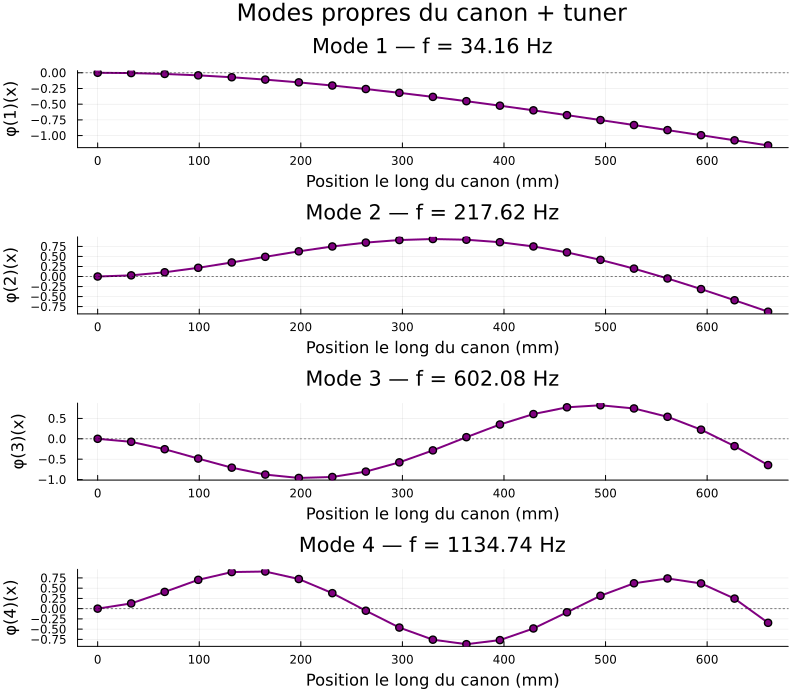
\includegraphics[width=0.85\linewidth]{plot_modes_propres.png}
		\caption{First four mode shapes $\phi_n(x)$ of the barrel fitted with a 200\,g tuner (FEM calculation, 20 elements). Note the monotonic shape of mode 1 (spatial antinode at the muzzle), and the progressive migration of the spatial nodes of higher modes toward the muzzle, a consequence of mass concentration at $x=L$.}
		\label{fig:modes_propres}
	\end{figure}

	\subsection{Sensitivity via the Rayleigh quotient}
	\label{sec:rayleigh}

	The \emph{Rayleigh quotient} associated with mode $n$ reads
	\begin{equation}
		\omega_n^2 \;=\; \frac{\{\phi_n\}^{\!\top}[K]\{\phi_n\}}{\{\phi_n\}^{\!\top}[M]\{\phi_n\}}.
	\end{equation}
	Let $\phi_n^{(L)}$ denote the mode component at the muzzle node (in translation). A perturbation $\delta m_t$ of the tuner mass modifies $[M]$ by $\delta m_t\,\phi_n^{(L)\,2}$ in the denominator, without affecting $[K]$. To first order, we obtain:
	\begin{equation}
		\label{eq:dwdmt}
		\boxed{\;\frac{\mathrm{d}\omega_n^2}{\mathrm{d}m_t} \;\approx\; -\,\omega_n^2\,\frac{\big|\phi_n^{(L)}\big|^2}{\{\phi_n\}^{\!\top}[M]\{\phi_n\}}\;\le 0.\;}
	\end{equation}
	Two important conclusions follow:
	\begin{enumerate}
		\item Adding mass at the muzzle \emph{always lowers} the frequency (negative sign).
		\item The reduction is more pronounced when the mode has a large amplitude at the muzzle. For the fundamental mode of a cantilever beam, $\phi_1^{(L)}$ is maximum, so $f_1$ drops strongly; for mode 2, the vibrational node moves closer to the muzzle, and the tuner's effect is more modest.
	\end{enumerate}
	These properties form the basis of the tuning mechanism: by moving the position of a sliding mass (or stacking weights), the shooter continuously sweeps $f_1$ over a typical range of $\pm 15$ to $\pm 30\,\%$.

	\subsection{Modal decomposition and transient response}

	By decomposing the response onto the basis of mass-normalised mode shapes, $\{u(t)\} = \sum_n q_n(t)\{\phi_n\}$, equation \eqref{eq:dynsemi} decouples into
	\begin{equation}
		\ddot q_n(t) + 2\zeta_n \omega_n\, \dot q_n(t) + \omega_n^2\, q_n(t) \;=\; f_n(t),\quad f_n(t) = \{\phi_n\}^{\!\top}\{F(t)\}.
	\end{equation}
	For an impulsive excitation (the pressure+projectile signature resembles a pulse of a few hundred microseconds), each mode begins a free oscillatory regime. The global rotational response at the muzzle is then
	\begin{equation}
		\theta(L,t) \;=\; \sum_n \phi_n^{\theta(L)}\, q_n(t),
	\end{equation}
	where $\phi_n^{\theta(L)}$ is the rotation component of mode $n$ at the muzzle node. In practice, the first mode dominates the muzzle kinematics at characteristic times $\sim t_b$; it is therefore essentially its tuning that the tuner targets.

	\paragraph{A transient regime, not an established standing wave.} A caveat is in order, one that Kolbe~\cite{KolbeSim} makes the heart of his argument: it is tempting to represent ``how a barrel vibrates'' by the \emph{analytic standing-wave solutions} of the beam equation. Yet these waves do \emph{not} form during the useful window. Their phase velocity is too low for a steady standing-wave regime to establish itself over the $t_b \approx 1$--$3$~ms of bullet passage: at that instant the barrel is still within the \emph{transient response} to the impulsive recoil moment, not in a settled periodic regime. This is precisely why the modal decomposition above is exploited here as a \emph{forced transient response} (integrated step by step by Newmark-$\beta$) rather than as a superposition of modes with frozen amplitudes, and why the reasoning of Section~\ref{sec:nodes} favours the \emph{temporal node} (the instantaneous state of the oscillation at $t_b$) over the spatial node (a property of a fully established mode).

	\section{Muzzle kinematics and positive compensation}
	\label{sec:cinematique}

	\subsection{Travel time and muzzle angle}

	Let $v(x,t)$ denote the projectile velocity at position $x$; the exit time is
	\begin{equation}
		t_b \;=\; \int_0^L \frac{\mathrm{d}x}{v(x)}.
	\end{equation}
	The effective launch angle at exit reads
	\begin{equation}
		\theta_\text{out} \;=\; \theta(L, t_b) \;=\; \left.\frac{\partial y}{\partial x}\right|_{x=L,\,t=t_b}.
	\end{equation}
	A variation $\Delta \theta_\text{out}$ produces a vertical displacement on target (at distance $D$, to first order without ballistic correction):
	\begin{equation}
		\Delta h \;\approx\; D\,\Delta \theta_\text{out}.
	\end{equation}
	The underlying geometry is that of figure~\ref{fig:compensation_positive} in the introduction: what section~\ref{sec:intro} described qualitatively is here reformulated in terms of muzzle angle and on-target effect.

	\subsection{Coupling between velocity spread and vertical dispersion}
	\label{sec:couplage}

	A variation $\Delta v_0$ of the muzzle velocity induces two cumulative effects:
	\begin{enumerate}
		\item \emph{Additional ballistic drop.} At distance $D$, for a flat trajectory, the drop below line of sight is $h_\text{bal}(v_0) \simeq g D^2/(2 v_0^2)$, hence
		\begin{equation}
			\label{eq:dhbal}
			\frac{\partial h_\text{bal}}{\partial v_0} \;\simeq\; -\,\frac{g D^2}{v_0^3} \;<\;0.
		\end{equation}
		Numerically, at $D=50$\,m and $v_0 \approx 318$\,m/s (1043 ft/s, Eley Tenex), $\partial h_\text{bal}/\partial v_0 \approx -0.76$\,mm/(m/s), i.e.\ $-0.016$ MOA per ft/s: exactly the number computed by Kolbe~\cite{Kolbe} using a trajectory solver. The choice of $v_0$ matters and must remain \emph{consistent} with the ammunition on which $\tau_v$ was measured (Eley Tenex, see below): at $v_0 = 308$\,m/s one would obtain $-0.0176$ MOA per ft/s, 10\,\% too high, and the error would propagate all the way to criterion \eqref{eq:dthetaopt}.
		\item \emph{Exit-time shift.} The internal kinematics couples $t_b$ and $v_0$: in the limit, $t_b \propto 1/v_0$ gives $\partial t_b/\partial v_0 = -t_b/v_0$, but the actual dependence is stronger because a more energetic charge raises the pressure \emph{throughout} the bore and shortens $t_b$ more than a simple kinematic ratio. We therefore write
		\begin{equation}
			\tau_v \;\equiv\; -\,\frac{\partial t_b}{\partial v_0} \;>\; 0,
		\end{equation}
		a quantity directly measurable using a chronograph coupled to a muzzle-exit sensor. Kolbe reports~\cite{Kolbe}, for Eley Tenex in a 26" barrel,
		\begin{equation}
			\tau_v \;\approx\; \frac{1\ \text{ms}}{375\ \text{ft/s}} \;=\; \frac{1\ \text{ms}}{114\ \text{m/s}} \;\approx\; 8.8\ \mu\text{s\,/\,(m/s)},
		\end{equation}
		and argues that this value is, to within $\pm 10\,\%$, a constant for rimfire barrels longer than 6 inches.
	\end{enumerate}
	The positive-compensation condition requires the two contributions to cancel on target:
	\begin{equation}
		\label{eq:compensation}
		\boxed{\;\frac{\mathrm{d}\theta_\text{out}}{\mathrm{d}t}\bigg|_{t_b}\cdot \Delta t_b \;+\; \frac{1}{D}\frac{\partial h_\text{bal}}{\partial v_0}\Delta v_0 \;=\; 0.\;}
	\end{equation}
	Substituting $\Delta t_b = -\tau_v\,\Delta v_0$ and \eqref{eq:dhbal}, we obtain the \emph{optimal angular velocity} at the muzzle at the moment of exit:
	\begin{equation}
		\label{eq:dthetaopt}
		\dot \theta_\text{out}^\star \;=\; \frac{1}{D\,\tau_v}\,\frac{\partial h_\text{bal}}{\partial v_0} \;=\; -\,\frac{g\,D}{v_0^3\,\tau_v}.
	\end{equation}
	\emph{The negative signs of $\partial h_\text{bal}/\partial v_0$ and $\partial t_b/\partial v_0$ combine to make $\dot\theta_\text{out}^\star$ positive: the muzzle must therefore be rising ($\dot\theta>0$) at the moment of shot release.} Numerically, with $D=50$\,m, $v_0 = 318$\,m/s and $\tau_v = 8.8\,\mu$s/(m/s):
	\begin{equation*}
		\dot\theta_\text{out}^\star \;\approx\; 1.73\ \text{mrad/ms} \;\approx\; 5.96\ \text{MOA/ms},
	\end{equation*}
	to be compared with the $6.0$ MOA/ms experimentally measured by Kolbe: \emph{the agreement is better than} $1\,\%$. This is not fortuitous --- the two routes are independent. Kolbe multiplies his measured natural drop ($0.016$ MOA per ft/s) by his exit-time sensitivity ($375$ ft/s per ms); we start from the ballistic kinematics \eqref{eq:dhbal} and $\tau_v$. That the two converge to within $1\,\%$ validates the chain of reasoning --- provided $v_0$ is kept consistent with the reference ammunition.

	\subsection{Spatial node \emph{vs} temporal node: a semantic clarification}
	\label{sec:nodes}

	The vocabulary of \emph{node} and \emph{antinode}, inherited from the acoustics of standing waves, often causes confusion when applied to shooting. Two physically distinct meanings coexist:

	\paragraph{Spatial node/antinode} --- special points of the \emph{mode shape} $\phi_n(x)$ along the barrel: a \emph{spatial node} is an $x^\star$ such that $\phi_n(x^\star)=0$ (zero transverse displacement); a \emph{spatial antinode} is an $x^\star$ where $|\phi_n|$ reaches a local maximum. For the fundamental mode of a cantilever beam, the shape is monotonically increasing from 0 (clamped end) to $\phi_1(L)$ (muzzle). \textbf{The muzzle is therefore, by construction, a spatial antinode of mode 1.} No choice of tuner moves this property: the muzzle remains where the bullet exits, at $x=L$.

	Higher modes ($n\ge 2$), on the other hand, exhibit spatial nodes \emph{inside} the barrel. Placing the tuner precisely at a spatial node of mode $n$ makes that mode insensitive to the added mass (cf.\ generalisation of \eqref{eq:dwdmt} to a mass positioned away from $x=L$). This is the trick of so-called \emph{harmonically-balanced} tuners: $f_1$ can be adjusted without disturbing $f_2$ or $f_3$, which makes the adjustment more monotonic and reproducible.

	\paragraph{Temporal node/antinode} --- special points of the \emph{in-time} oscillation of the muzzle angle $\theta(L,t)$: a \emph{temporal node} is an instant $t^\star$ where $\theta(L,t^\star)=0$ (zero crossing); a \emph{temporal antinode} is an instant where $|\theta(L,t)|$ reaches a maximum (i.e.\ $\dot\theta(L,t^\star)=0$). For a nearly sinusoidal mode 1, these two types of instants alternate at a quarter period.

	The criterion \eqref{eq:dthetaopt} then translates unambiguously:
	\begin{center}
	\begin{tabular}{lcc}
		\toprule
		Exit instant $t_b$ & $\theta(L,t_b)$ & $\dot\theta(L,t_b)$ \\
		\midrule
		\textbf{Temporal antinode} & $\pm\Theta_1$ (max) & $0$ \\
		\textbf{Temporal node} & $0$ & $\pm\Theta_1\,\omega_1$ (max) \\
		\bottomrule
	\end{tabular}
	\end{center}

	\textbf{Positive compensation requires exit in the vicinity of an \emph{ascending temporal node}}, where $\theta = 0$ and $\dot\theta > 0$ is at its maximum. Exiting at the peak of the oscillation (temporal antinode) is, on the contrary, the \emph{worst} case: not only does $\dot\theta=0$ wipe out any compensation, but one also fires with a maximum static angular offset that shifts the mean point of impact.

	\begin{figure}[!htb]
		\centering
		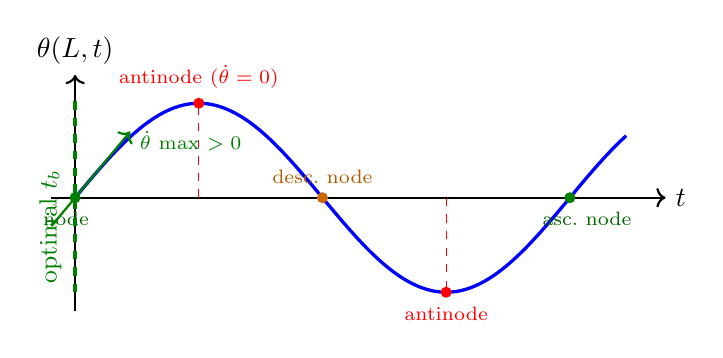
\begin{tikzpicture}[x=1.0cm, y=1.2cm]
			% Axes
			\draw[->, thick] (-0.3, 0) -- (7.5, 0) node[right] {$t$};
			\draw[->, thick] (0, -1.2) -- (0, 1.3) node[above] {$\theta(L,t)$};
			% Sinusoid
			\draw[blue, very thick, domain=0:7, samples=200, smooth]
				plot (\x, {sin(\x r)});
			% Ascending temporal nodes (green)
			\fill[green!50!black] (0, 0) circle (2pt);
			\fill[green!50!black] (6.283, 0) circle (2pt);
			% Descending temporal node (orange)
			\fill[orange!80!black] (3.141, 0) circle (2pt);
			% Temporal antinodes (red)
			\fill[red] (1.571, 1) circle (2pt);
			\fill[red] (4.712, -1) circle (2pt);
			% Dashed lines
			\draw[red, dashed, thin] (1.571, 0) -- (1.571, 1);
			\draw[red, dashed, thin] (4.712, 0) -- (4.712, -1);
			% Annotations
			\node[red, above] at (1.571, 1.05) {\scriptsize antinode ($\dot\theta = 0$)};
			\node[red, below] at (4.712, -1.05) {\scriptsize antinode};
			\node[green!40!black, anchor=north east] at (0.3, -0.05)
				{\scriptsize node};
			\node[green!40!black, anchor=north] at (6.5, -0.05)
				{\scriptsize asc.\ node};
			\node[orange!70!black, anchor=south] at (3.141, 0.05)
				{\scriptsize desc.\ node};
			% Optimal t_b
			\draw[green!50!black, very thick, dashed]
				(0, -1.0) -- (0, 1.1);
			\node[green!50!black, anchor=south east, rotate=90] at (-0.05, 0.4)
				{\small optimal $t_b$};
			% Tangent at t=0 (max ascending velocity)
			\draw[green!50!black, thick, ->] (-0.3, -0.3) -- (0.7, 0.7);
			\node[green!50!black, anchor=west] at (0.7, 0.6)
				{\scriptsize $\dot\theta$ max $> 0$};
		\end{tikzpicture}
		\caption{Temporal node vs antinode distinction on the muzzle angle $\theta(L,t)$. Positive compensation requires $t_b$ to fall in the vicinity of an \emph{ascending temporal node} (green point at $t=0$ and $t = T_1$), where $\theta = 0$ but $\dot\theta$ is maximum and positive. Exiting at a temporal antinode (red points, $\dot\theta = 0$) cancels the compensation.}
		\label{fig:noeud_temporel}
	\end{figure}

	What Kolbe~\cite{Kolbe,KolbeWeb} calls the ``upward swing of the vibration at the muzzle'' corresponds precisely to this \emph{ascending temporal node}. In the competitor jargon (\emph{ladder} or \emph{OCW}~\cite{Audette} method), the ``node'' of tuning refers more loosely to a zone of \emph{robustness} of grouping, i.e.\ a plateau around which a small shift of $t_b$ does not degrade the group. In the strict sense of vibration mechanics, this plateau is precisely the window around an ascending temporal node --- where $\ddot\theta(L,t_b)$ is close to zero and $\dot\theta(L,t_b)$ hovers near its extremal value, which makes the tuning weakly sensitive to fluctuations of $t_b$.

	\subsection{Experimental confirmation (Kolbe, 2015)}

	Kolbe~\cite{KolbeWeb} directly verified the criterion \eqref{eq:dthetaopt} on an instrumented test bench measuring the muzzle angle optically (crossed polariser) with a photo-detector gate locating the exact exit instant. On a 26" Border barrel, .22 LR calibre, Eley EPS Tenex ammunition, two configurations are compared:
	\begin{center}
	\begin{tabular}{lcc}
		\toprule
		Configuration & measured $\dot\theta(L,t_b)$ & On-target groups \\
		\midrule
		Bare barrel & $-9.4$ MOA/ms (muzzle dropping) & pronounced \emph{vertical} string \\
		Barrel + 200 g tuner & $+6.0$ MOA/ms (muzzle rising) & \emph{round} groups \\
		\bottomrule
	\end{tabular}
	\end{center}
	The value $+6.0$ MOA/ms coincides with criterion \eqref{eq:dthetaopt} for 50 m and the ammunition used. The near-complete elimination of vertical stringing experimentally confirms that the criterion is not only necessary (sign) but also sufficient (magnitude) when higher-order modes remain weakly excited.

	In particular, Kolbe notes that the \emph{vertical translation velocity} $\dot y(L,t_b)$ of the muzzle contributes negligibly to the on-target dispersion compared to $\dot\theta(L,t_b)$: it is indeed the muzzle's \emph{rotation}, not its translation, that determines the effective launch angle. This observation justifies \emph{a posteriori} the DOF split (translation + rotation) of the FEM model, and orients the control toward extracting the rotational component at the terminal node.

	\subsection{Validation by FEM + Newmark-$\beta$ simulation}
	\label{sec:validation_num}

	The \texttt{Julia} simulator accompanying this document (\texttt{simulation.jl}) implements the full formalism: FEM assembly, clamping, tuner, internal ballistics (``burnout'' profile: acceleration over a fraction $\phi=0.35$ of the barrel, then coast, calibrated on Kolbe's $\tau_v$), excitation by the breech recoil moment $M(t) = p(t)\,A_\text{bore}\,h_\text{offset}$, moving projectile load, Rayleigh damping and Newmark-$\beta$ scheme. The lever arm $h_\text{offset}$ is automatically calibrated on an amplitude peak of $\sim 10$ MOA/ms. This peak value is a \emph{scale choice} of ours, not a figure from Kolbe: he publishes no oscillation peak, only the rate \emph{at the instant of exit} ($-9.4$ MOA/ms bare barrel, $+6.0$ tuned). The only quantity confronted with measurement is therefore $\dot\theta(L,t_b)$, not the peak.

	\begin{figure}[!htb]
		\centering
		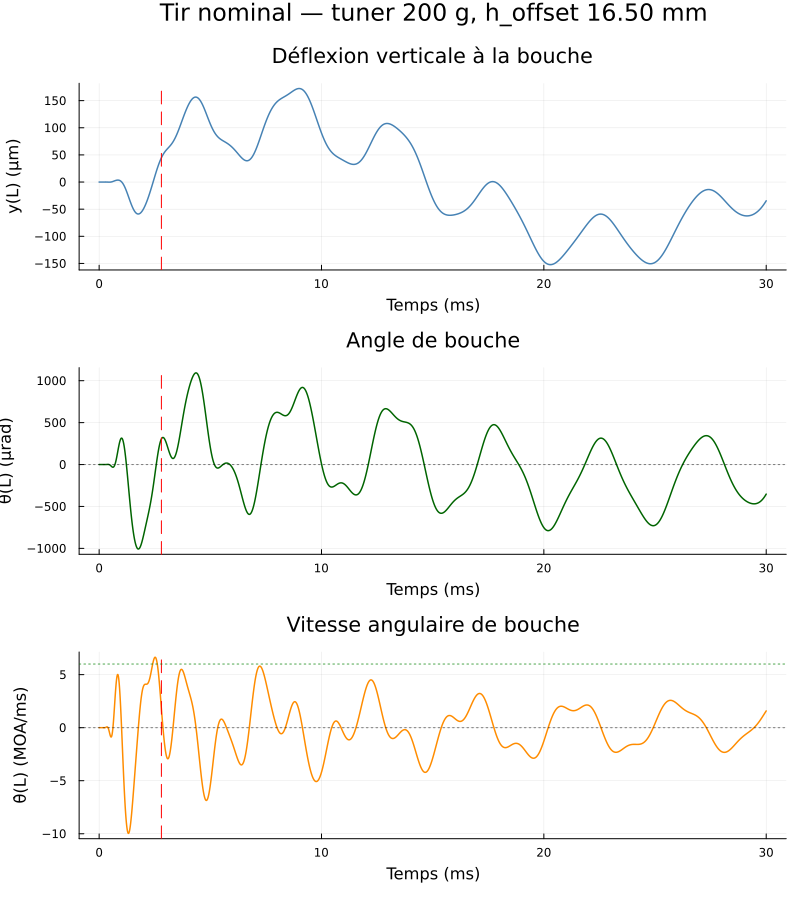
\includegraphics[width=0.85\linewidth]{plot_tir_nominal.png}
		\caption{Simulated transient response for the nominal configuration (200\,g tuner, $h_\text{offset} = 16.5$ mm). From top to bottom: deflection $y(L,t)$, muzzle angle $\theta(L,t)$, and angular velocity $\dot\theta(L,t)$. The red dashed line marks $t_b = 2.80$ ms (burnout profile); the green dotted line indicates the Kolbe target (6 MOA/ms). At $t_b$ the model gives $\dot\theta = +1.8$ MOA/ms: of the right sign (rising, tuner fitted) but of amplitude below the target --- see the caveat below.}
		\label{fig:reponse_transitoire}
	\end{figure}

	\begin{figure}[!htb]
		\centering
		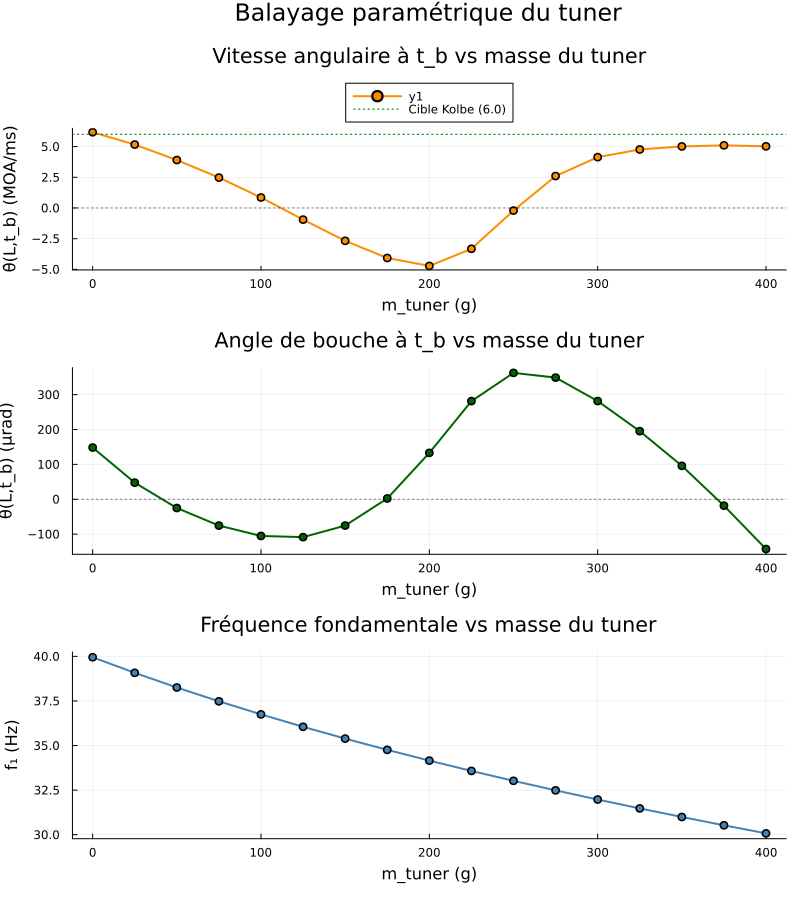
\includegraphics[width=0.85\linewidth]{plot_balayage_tuner.png}
		\caption{Parameter sweep on the tuner mass $m_t \in [0, 400]$\,g (other parameters fixed). From top to bottom: (i)~$\dot\theta(L,t_b)$ \emph{changes sign} --- $-1.1$ MOA/ms for the bare barrel (muzzle descending at exit) toward $+2.6$ at 400\,g (rising): this is Kolbe's mechanism, the tuner taking the muzzle from descending to rising; (ii)~$\theta(L,t_b)$ decreases monotonically from $+416$ to $+205$ µrad, reflecting a shift of the mean point of impact; (iii)~$f_1$ decreases monotonically from 39.9 to 30.3 Hz (relation predicted by the Rayleigh quotient, equation \eqref{eq:dwdmt}).}
		\label{fig:balayage_tuner}
	\end{figure}

	\paragraph{The internal-ballistics profile now reproduces $\tau_v$.} The ``burnout'' profile (constant acceleration over a fraction $\phi = 0.35$ of the barrel, then coast) realises $\tau_v = -\partial t_b/\partial v_0 = (1+\phi)\,L/v^2 = 8.8\ \mu$s/(m/s), exactly the value measured by Kolbe and used in criterion \eqref{eq:dthetaopt}. The former exponential lag $v = v_m(1-e^{-t/\tau})$ was \emph{front-loaded} (all acceleration at the breech, then coast): its sensitivity capped at $L/v^2 \approx 6.5\ \mu$s, 35\,\% too low, the bullet exiting too early ($t_b = 2.46$ vs $2.80$~ms). Kolbe's kinematic chain --- natural drop, exit-time sensitivity, required rate --- is thus \emph{fully} reproduced (\texttt{kolbe\_validation.jl}: $0.016 \times 375 = 6.0$ MOA/ms recovered to $1\,\%$).

	What remains out of reach is the \emph{absolute amplitude}. At the correct exit time $t_b = 2.80$~ms, the clamped model gives $\dot\theta(L,t_b)$ of the right \emph{sign} --- negative for the bare barrel ($\approx -1.1$ MOA/ms, muzzle descending, like Kolbe's measured $-9.4$), brought toward positive by the muzzle mass ($+2.6$ at 400\,g) --- but about three times too small to reach the measured $6.0$ MOA/ms without an implausible vibration amplitude. This is the symptom, already encountered, of the \emph{rigid-body rotation} absent from the clamped model, not a defect of the ballistic profile. Notably, correcting the profile \emph{improves} the qualitative agreement: at the former $t_b = 2.5$~ms the bare barrel came out \emph{rising} (wrong sign); at the correct time it comes out \emph{descending}, consistent with Kolbe.

	This amplitude deficit has since been \emph{lifted} by the free-recoiling rifle model (\texttt{harral\_rifle\_sweep.jl}, \texttt{kolbe\_amplitude.jl}): with the physically anchored recoil moment ($\int A_\text{bore}\,p\,dt = (1+\beta)\,m_p\,v$), the peak of $|\dot\theta|$ reaches $\sim 5$ MOA/ms for a one-inch bore height, $\sim 10$ for two inches --- Kolbe's order of magnitude, with no fitting parameter. Yet the rigid-body rotation contributes only $\sim 0.2$ MOA/ms: it is not what supplies the amplitude, but the elastic \emph{whip} it excites once the breech is freed. Only the \emph{exact} match of $\dot\theta(L,t_b)$ --- its phase at exit --- remains out of reach, depending on the real whip frequency and exit time, which are unpublished.

	These plots illustrate a distinction essential for the shooter: the tuner acts \emph{primarily on the mean point of impact} (via $\theta(L,t_b)$) and \emph{secondarily on the vertical dispersion} (via $\dot\theta(L,t_b)$). When $t_b \ll T_1$, the optimality window in $\dot\theta$ is wide and flat; the tuner adjustment then mainly serves to compensate for the velocity spread, while the sight adjustment takes care of the POI shift.

	\section{Practical conclusions for the shooter}
	\label{sec:conclusions}

	The preceding formalism, validated numerically by the finite-element simulation, leads to several exploitable conclusions.

	\paragraph{1. Effect of a muzzle mass.} Adding a mass at the muzzle \emph{lowers} the fundamental frequency (cf.\ \eqref{eq:dwdmt}). For the reference barrel, the adjustment range of a 100--400\,g tuner covers an $f_1$ variation of the order of $8$ to $24\,\%$ (39.9\,Hz $\to$ 30.3\,Hz). The equivalent temporal shift in the vibration cycle is of the order of a fraction of a millisecond, which suffices to sweep the entire optimality window in which $t_b \approx 2$--$3$\,ms must be positioned.

	\paragraph{2. Direction of adjustment.} Extending the effective tuner position (screwing it outward) increases $J_t$ and the lever arm, which amplifies the mass effect and lowers $f_1$. This is the action that ``slows down'' the muzzle kinematics and delays the zero crossing of $\theta(L,t)$: useful for slower ammunition (delayed exit $t_b$).

	\paragraph{3. Sensitivity to ammunition.} Any change of lot or brand modifies $\bar v$ and therefore $t_b$. The optimality window ($\dot\theta_\text{out}$ near $\dot\theta^\star_\text{out}$) is narrow: a 0.1 ms shift on $t_b$ may represent a non-negligible fraction of the period $T_1 = 2\pi/\omega_1$. Any new lot must therefore be the subject of a systematic retuning at the tuner notch (\emph{ladder tune} or \emph{Audette} method).

	\paragraph{4. Physical limits.} The tuner does not remove the intrinsic dispersion of the ammunition: it converts a vertical dispersion into a genuinely tighter group only if \eqref{eq:compensation} is satisfied to within a few MOA/ms. The horizontal dispersion, independent of the ($\Delta v_0,\, \theta_\text{out}$) pair, is not compensated. The expected on-target gain therefore remains bounded by the other error sources (wind, bullet imbalance, parallax, sight).

	\paragraph{5. Robustness to higher modes.} Modes 2 and 3, of significantly higher frequencies (cf.\ the previous table), produce a fast oscillation superposed on $\theta(L,t)$. If they are poorly damped and significantly excited, they create a residual variability (\emph{flyers}) even after tuning. A muzzle mass distinct from an integer harmonic of mode 1 (anti-resonance) helps filter them out, which motivates the ``adjustable'' double-ring designs.

	\paragraph{6. Range of validity: centerfire \emph{vs} rimfire.} A caveat of intellectual honesty, stated by Kolbe himself~\cite{KolbeSim}, deserves to be reported. The \emph{principle} of positive compensation (Sections~\ref{sec:intro} and~\ref{sec:cinematique}) is general and was first established for rimfire. The \emph{impulsive recoil-moment excitation model} adopted here (and in Kolbe's simulator), however, is chiefly relevant to \emph{centerfire} calibres: there the pressure--time curve is long ($\sim 1$~ms, peak $\sim 350$~MPa $\approx 50{,}000$~psi, .308~Win-like profile) and the recoil high, so that the recoil moment does dominate the onset of vibration. For the \emph{.22~LR}, the pressure pulse is so brief that, according to Kolbe, the recoil moment alone reproduces the observed vibrations poorly: \emph{other} excitation sources (rifling engagement, the moving projectile's weight effect, assembly play) take a comparable share. Our model captures them partially --- this is the very purpose of contributions (b) and (c) of Section~\ref{sec:excitation}, absent from Kolbe's original simulator --- but the rimfire numbers given in this document should be read as \emph{calibrated orders of magnitude}, not absolute predictions. Direct experimental validation (Section~\ref{sec:validation_num}) remains the reference for rimfire.

	\paragraph{7. A planar model: vertical vibration only.} A second caveat of intellectual honesty concerns the dimensionality of the model. The whole preceding development is \emph{planar}: the Euler--Bernoulli beam \eqref{eq:EB} is solved in a single plane and describes only the \emph{vertical} component of the muzzle oscillation. Nothing, however, forces the barrel to vibrate only vertically: in reality the muzzle traces a \emph{two-dimensional orbit} (an elliptical ``whip''), and its horizontal component --- already noted as uncompensated in point~4 --- is corrected by no positive-compensation mechanism. It adds to the residual dispersion and sets a floor on the achievable precision. If the vertical model nonetheless remains relevant to first order, it is because \emph{two effects break the symmetry} and privilege the vertical plane: \emph{gravity}, which imposes a static sag and orients the dominant mode; and the \emph{recoil geometry}, whose muzzle-rise couple (bore above the centre of gravity, Section~\ref{sec:intro}) is essentially vertical. Above all, positive compensation \eqref{eq:compensation} does not require the vibration to be \emph{purely} vertical: it suffices that the vertical component of the muzzle angle correlate, in the right direction, with the exit time $t_b$ (hence with the muzzle velocity). The horizontal motion adds noise without destroying this benefit, which the empirical success of tuners in .22~LR benchrest confirms. The planar model is therefore a \emph{first-order} model: useful and predictive, but which structurally underestimates the real dispersion.

	\paragraph{8. A distance-specific tuning.} The optimal angular velocity \eqref{eq:dthetaopt} is \emph{proportional to the shooting distance}: $\dot\theta_\text{out}^\star = -\,gD/(v_0^3\,\tau_v) \propto D$. A tuner tuned for $D = 50$~m therefore realises equality \eqref{eq:compensation} only at that distance; at another distance, the ballistic term (in $\partial h_\text{bal}/\partial v_0 \propto D^2$) and the angular term (in $\dot\theta_\text{out}\,D$) no longer cancel exactly and the compensation becomes \emph{partial} --- under-compensation beyond the tuning distance, over-compensation short of it ---, the velocity dispersion gradually reappearing as vertical stringing. The lesson is that positive compensation does not \emph{reduce} the muzzle-velocity dispersion of the lot (the velocity standard deviation is unchanged): it \emph{masks} its vertical effect, and only near the tuning distance. A lot with a low velocity standard deviation therefore remains preferable, and a tuner is best verified at the competition distance. The phenomenon is nonetheless gradual: a setting established at short range retains part of its benefit at longer range as long as the intrinsic group remains smaller than the ballistic stringing it corrects.

	\paragraph{9. A tuner is not always beneficial: Harral's FEA study.} A final caveat, an empirical one, comes from an independent finite-element simulation carried out by A.\ Harral~\cite{Harral} on a .22~LR benchrest rifle (``Esten's'' rifle). Computing, for the velocity range 1035--1075~fps, the on-target vertical spread with and without a muzzle mass, Harral obtains a counter-intuitive result: the \emph{best} vertical group here is obtained \emph{without} a tuner ($0.091$~inch, i.e.\ $\approx 2.3$~mm), adding a mass \emph{degrading} it monotonically --- $0.122$~inch ($\approx 3.1$~mm) with 4.9~oz ($\approx 139$~g), $0.183$~inch ($\approx 4.6$~mm) with 16~oz ($\approx 454$~g). The interpretation is consistent with our formalism: this bare barrel already places, by its geometry (a flexible \emph{reverse-taper} profile), the bullet exit $t_b$ on a favourable \emph{ascending} flank of $\theta(L,t)$; adding muzzle weight slows the kinematics \eqref{eq:dwdmt} and drifts $t_b$ toward a \emph{descending} flank, where the combination becomes additive (dispersion \emph{worsened}). Two practical lessons follow: (i) the tuner does not \emph{create} compensation, it merely \emph{shifts} $t_b$ within the vibration cycle --- if the barrel is already well placed, the best tuner position may be ``no mass'', its role reducing to \emph{re-tuning} after a change of lot or distance (point~3 and point~8); (ii) a \emph{light} mass, with finer adjustment, is preferable to a heavy one that risks ``overflying'' the optimum from one notch to the next. Harral further confirms, in the same study, the distance-specific character (point~8): a setting made at 50~yd does not remain optimal at 100~yd.

	\emph{A caveat on this warning.} All of the above rests on a \emph{single, purely numerical} source. Kolbe~\cite{KolbeSim} --- who did measure --- considers that work unconfirmed: ``His work has lacked the experimental confirmation needed to verify his computer modelling, however.'' Harral publishes neither his rifle data (a single figure: 10.5~lb), nor his natural frequencies, nor his damping. The result remains plausible and consistent with the formalism, but must be read as an \emph{unvalidated simulation prediction}, not as a measured fact.

	\paragraph{10. In a vice or at the shoulder? The support condition \emph{is} the mechanism.} The most common practical question --- should one tune with the rifle clamped in a vice, to ``remove the human factor''? --- calls for a blunt answer: \emph{no}, and not for reasons of realism, but because a rigid vice \emph{suppresses the very phenomenon one is trying to tune}. The driving moment \eqref{eq:moment_recul} exists only because the rifle \emph{recoils and pivots about its centre of gravity} (section~\ref{sec:excitation}); rigidly clamping the base cancels that term, leaving only elastic bending of the tube, which produces \emph{no} compensation at all. Kolbe's own test rig was a clamp --- but he points out that it was not rigid: ``The relatively thin base plate flexed under recoil and allowed the barrel clamp to rotate backwards, resulting in an upwards vertical muzzle flip.'' A truly rigid clamp would have shown nothing. For \emph{benchrest}, the matter is settled: shooting off bags is, in Kolbe's words, ``a fair approximation'' of the free recoil the model assumes. For \emph{shouldered or prone shooting}, however, shouldering adds effective mass and constrains the rotation: since the amplitude scales as $h_\text{cg}/m_r$ \eqref{eq:hoffset_phys}, a tune established in free recoil has no reason to remain optimal when shouldered. Kolbe is cautious (``if a small calibre rifle is gripped tightly or pulled hard into the shoulder then the recoil dynamics could be affected'') and did not measure it. On present knowledge the prudent rule is therefore: \emph{tune in the position you shoot}, and re-check the tune if you change position or hold.

	\section*{Bibliography}

	\begin{thebibliography}{9}

		\bibitem{Rao}
		S. S. Rao, \textit{Mechanical Vibrations}, Pearson, 2017.

		\bibitem{Meirovitch}
		L. Meirovitch, \textit{Elements of Vibration Analysis}, McGraw-Hill, 1986.

		\bibitem{Bathe}
		K.-J. Bathe, \textit{Finite Element Procedures}, 2nd ed., Prentice Hall, 2014.

		\bibitem{Carlucci}
		D. Carlucci and S. Jacobson, \textit{Ballistics: Theory and Design of Guns and Ammunition}, 3rd ed., CRC Press, 2018.

		\bibitem{Kolbe}
		G. Kolbe, \textit{Using barrel vibrations to tune a barrel --- The Vibrations of a Barrel Tuned for Positive Compensation}, Border Barrels, 2015.

		\bibitem{KolbeWeb}
		G. Kolbe, \textit{The Vibrations of a Barrel Tuned for Positive Compensation} (online article, updated 18 November 2015),\\
		\url{http://www.geoffrey-kolbe.com/articles/rimfire_accuracy/tuning_a_barrel.htm}.

		\bibitem{KolbeSim}
		G. Kolbe, \textit{Barrel Vibrations Simulator} (``lumped parameter'' finite-element model and modelling notes, online, accessed June 2026),\\
		\url{http://www.geoffrey-kolbe.com/articles/rimfire_accuracy/barrel_vibrations.htm}.

		\bibitem{Mallock}
		A. Mallock, \textit{Vibrations of Rifle Barrels}, Proceedings of the Royal Society, Vol.~68, p.~327, 1901.\\
		\url{https://www.tireur.org/articles/Mall01.pdf}.

		\bibitem{Audette}
		C. Audette, \textit{The Optimum Charge Weight (OCW) Method}, \textit{Precision Shooting Magazine}, 2005--2010.

		\bibitem{Harral}
		A. Harral, \textit{Al's 22LR --- Barrel Tuner Analysis} (finite-element study of a muzzle tuner on a .22~LR benchrest rifle, online, accessed July 2026),\\
		\url{https://varmintal.com/a22lr.htm}.

		\bibitem{Newmark}
		N. M. Newmark, \textit{A Method of Computation for Structural Dynamics}, ASCE Journal of the Engineering Mechanics Division, 85(3), pp.\ 67--94, 1959.

	\end{thebibliography}

\end{document}
